\documentclass{article}
\usepackage{graphicx} % Required for inserting images
\usepackage{amsmath}
\usepackage{amssymb}
\usepackage[italian]{babel}
\usepackage{listings}
\usepackage{tikz}
\usepackage{float}
\usetikzlibrary{graphs}
\usepackage[algoruled,vlined]{algorithm2e} % o opzioni diverse
% Oppure
% \usepackage{algorithmicx}
% \usepackage{algpseudocode}


\usepackage{amsthm}
\usepackage{hyperref}
%\usepackage[backend=biber,style=numeric]{biblatex}

% Definizione dell'ambiente per le definizioni
\newtheorem{definition}{Definizione}[section]
\newtheorem{proposition}{Proposizione}[section]
\newtheorem{theorem}{Teorema}[section]
\newtheorem{lemma}{Lemma}[section]


\title{Generazione casuale mediante catene di Markov}
\author{Andrea Alfonsi e Stefano Bucciarelli}
\date{\today}

\begin{document}

\maketitle
\newpage

\tableofcontents
\newpage

\section{Introduzione}

Questo documento riguarda i metodi Monte Carlo basati su Catena di Markov, cioè ad algoritmi utilizzati per il campionamento di distribuzioni di probabilità, che simulano una catena di Markov con una distribuzione stazionaria che corrisponde alla distribuzione desiderata. Nella prima parte del documento ripercorreremo le basi teoriche sulle catene di Markov, con particolare riferimento alle catene di Markov ergodiche, in quanto garantiscono l'effettiva convergenza alla distribuzione stazionaria. Successivamente andremo a teorizzare algoritmi per specifici problemi, definendo le rispettive catene di Markov e dimostrandone l'ergodicità, e infine implementeremo gli algoritmi e ne analizzeremo i risultati. 

\section{Richiami sulle catene di Markov}
% Parte iniziale sulle catene di markov
Uno spazio di probabilit\`a \`e una terna $(\Omega, \mathcal{F}, P)$ che soddisfa le seguenti propriet\`a: 

\begin{itemize}
    \item \textbf{$\Omega$} \`e un insieme, detto spazio campione (o universo dei risultati). I suoi elementi sono chiamati punti campione.
    \item \textbf{$\mathcal{F}$} \`e una $\sigma$-algebra su $\Omega$. Questa \`e una famiglia di sottoinsiemi di $\Omega$ che include:
    \begin{itemize}
        \item $\Omega$ stesso;
        \item Il complementare $A^c$ di ogni evento $A \in \mathcal{F}$;
        \item L'unione numerabile $\cup_{i \ge 1}A_i$ per ogni sequenza $\{A_i\}_{i \ge 1}$ di elementi di $\mathcal{F}$.
    \end{itemize}
    Gli elementi di $\mathcal{F}$ sono chiamati eventi.
    \item \textbf{$P$} \`e una misura di probabilità su $\mathcal{F}$. Si tratta di una funzione $P: \mathcal{F} \rightarrow [0,1]$ tale che:
    \begin{itemize}
        \item $P(\Omega) = 1$;
        \item Per ogni sequenza $\{A_i\}_{i \ge 1}$ di eventi disgiunti di $\mathcal{F}$, $P(\cup_{i \ge 1}A_i) = \sum_{i \ge 1} P(A_i)$ (additivit\`a numerabile).
    \end{itemize}
\end{itemize}

\noindent
Una \textbf{catena di Markov finita e omogenea} \`e definita da tre elementi principali:

\begin{itemize}
    \item Un insieme finito $E = \{S_1, S_2, \dots, S_N\}$ di elementi, chiamati \textbf{stati}.
    \item Una distribuzione di probabilit\`a \textbf{$\mu_0$} definita su $E$, chiamata distribuzione iniziale, che se definita nella seguente maniera:
    $$
    \mu_0\{y\} = \delta_{\{x\}}(y) = \begin{cases}
                                      1 & \text{for} \; x = y \\
                                      0 & \text{for} \; x \neq y
                                      \end{cases}
    $$
    la catena viene detta "uscente dallo stato $x$".
    \item Una matrice stocastica \textbf{$P$}, detta matrice di transizione. La matrice $M = [m_{i,j}]_{i,j \in 1 \ldots N} = [p(x,y)]_{x,y \in E}$ ha coefficienti $p(x,y) \ge 0$ per ogni $x,y \in E$, e la somma dei coefficienti su ogni riga \`e 1 ($\sum_{y \in E} p(x, y) = 1$ per ogni $x \in E$).
\end{itemize}

Una catena di Markov rispetto a una filtrazione $(\mathcal{F}_n)_{n\in \mathbb{N}}$ \`e una sequenza $\{X_n\}_{n \in \mathbb{N}}$ di variabili aleatorie a valori in $E$ tale che:

\begin{enumerate}
    \item Per ogni $y \in E$, la probabilit\`a dello stato iniziale \`e $P(X_0 = y) = \mu_0\{y\}$.
    \item \textbf{Propriet\`a di Markov }: per ogni $n > 0$, $x, y \in E$, la probabilit\`a di transizione al passo successivo dipende solo dallo stato corrente, non dalla storia precedente:
    \[
    P(X_{n+1} = y | A, X_n = x) = P(X_{n+1} = y | X_n = x) =: p(x ,y) \; \forall A \in \mathcal{F}_n 
    \]
\end{enumerate}


% Definizioni e proposizioni che servono per il capitolo MCMC
\noindent
Per le seguenti definizioni consideriamo uno spazio di probabilità $(\Omega, \mathcal{F}, P)$ che supporta una catena di Markov $X = (X_i)_{i \in \mathbb{N}}$ con distribuzione iniziale $\mu_0$ a valori nello spazio degli stati $E = \{S_1, \ldots, S_N\}$. \\

% \begin{definition}
%     \label{def:proprieta}
%     Una catena di Markov finita eredita le propriet\`a della matrice di transizione associata. Cos\`i diremo che la catena \`e irriducibile se la matrice P \`e irriducibile. In modo analogo si definiscono le catene primitive, quelle periodiche e aperiodiche.
% \end{definition}

% \begin{quote}
%     Ricordiamo che una matrice quadrata non negativa \( A = [a_{ij}] \) si dice \textbf{irriducibile} se per ogni coppia di indici \( i, j \), esiste un intero \( n > 0 \), tale che \( a_{ij}^{(n)} > 0 \).\\
%     Questo significa che, nel grafo associato ad \( A \), per ogni coppia di nodi \( i, j \), esiste un intero \( n > 0 \) tale che \( i \xrightarrow{n} j \) (cio\`e la lunghezza $n$ del cammino da $i$ a $j$, non può essere nulla).
% \end{quote}

\begin{definition}
\label{def:irriducibile}
Definita la seguente funzione 
$$F(y, x) = P_y\{\rho_x < \infty\}.$$
dove $\rho_x := \inf\{n \geq 1 : X_n = x\}.$ \\
 Allora la catena di Markov si definisce \textbf{irriducibile} se $F(y,x) > 0$ $\forall x, y \in E$ 
\end{definition} 

\begin{definition}
\label{def:aperiodica}
Il \textit{periodo} dello stato $x \in E$ è definito 
$$d(x) := \mathrm{gcd} \{m \geq 1 \,;\, p^{(m)}(x, x) > 0\}.$$

E la catena di Markov si definisce \textbf{aperiodica} se il periodo di ogni stato $x \in E$ è uguale a $1$

(Ricordiamo che $p^{(n)}(x, y) = P_x(X_n = y)$)
\end{definition}


%\begin{definition}
%\label{def:algebra}
%Diciamo che $x \in E$ è:
%\begin{itemize}
%    \item[(i)] \textit{transiente} se $F(x, x) < 1$;
%    \item[(ii)] \textit{ricorrente} se $F(x, x) = 1$.
%\end{itemize}
%\end{definition}
%
%\begin{definition}
%\label{def:algebra}
%Sia $x \in E$ uno stato ricorrente della catena di Markov $X$. Diciamo che:
%\begin{itemize}
%    \item[(i)] $x$ è \textit{positivamente ricorrente} se $E_x[\rho_x] < \infty$;
%    \item[(ii)] $x$ è \textit{nulla ricorrente} se $E_x[\rho_x] = \infty$.
%\end{itemize}
%\end{definition}
%
%\begin{definition}
%    Definiamo l'operatore $\hat{T}: \mathcal{P}(E) \rightarrow\mathcal{P}(E)$ nel seguente modo:
%    
%    \[
%    (\hat{T}\mu)(A) = \sum_{x \in E} \mu(\{x\}) \sum_{y \in A} p(x, y), \quad \forall A \in E
%    \]
%
%    Sia \( M \) la matrice di transizione associata alla catena di Markov in un insime finito di stati. Si è interessati all'esistenza e unicit\`a di un vettore non negativo \( \pi \) tale che
%    \[
%    M^*\pi = \pi.
%    \]
%\end{definition}
%
%\begin{definition}
%\label{def:algebra}
%
%(Misura di probabilità invariante). Una misura di probabilità invariante o una distribuzione stazionaria per la catena di Markov $X$ è una distribuzione di probabilità $\hat{\mu} \in P(E)$ tale che
%$$\hat{T} \hat{\mu} = \hat{\mu}$$
%\end{definition}

\begin{definition}
    \label{def:stazionaria}
    Sia $\mathcal{P}(E)$ lo spazio delle distribuzioni di probabilità su $E$ e definito l'operatore \[
    \mathcal{T}: \mathcal{P}(E) \rightarrow \mathcal{P}(E), \quad(\mathcal{T} \mu)(A)=\sum_{x \in E} \mu\{x\} \sum_{y \in A} p(x, y), \quad A \in \mathcal{E} .
\]
    Una \textbf{distribuzione stazionaria} o misura di probabilità invariante è una distribuzione di probabilità $\pi \in \mathcal{P}(E)$ tale che
    \[
    \mathcal{T} \pi = \pi
    \]

\end{definition}

\begin{definition}
    \label{def:reversibile}
    Una catena di Markov $\{X_n\}_n$, definita sullo spazio degli stati $E = \{S_1, \ldots, S_N\}$ con matrice di transizione $P = [p(x,y)]_{x,y \in E}$, si dice \textbf{reversibile} se esiste una distribuzione di probabilità $\pi \in \mathcal{P}(E)$ tale che per ogni $x, y \in E$ vale la relazione
    \[
    \pi\{x\} \, p(x,y) = \pi\{y\} \, p(y,x)
    \]
\end{definition}

%\begin{proposition}
%\label{def:algebra}
%Sia $X$ una catena di Markov irriducibile con valori in uno spazio finito. Allora essa è \textit{positivamente ricorrente}.
%
%\end{proposition}

\begin{proposition}
\label{prp:rev_staz}
Se $\pi$ è una distribuzione reversibile per una catena $\{X_n\}_{n}$, allora $\pi$ è anche una distribuzione stazionaria per $\{X_n\}_{n}$.
\end{proposition}
\begin{proof}
    Siano $E$ e $P = [p(x, y)]_{x,y \in E}$, rispettivamente, l’insieme degli stati e la matrice di transizione della catena. Poiché $\pi$ è una distribuzione reversibile, per ogni $y \in E$ abbiamo

    $$(\mathcal{T}\pi)\{y\} = \sum_{x \in E} \pi\{x\} p(x, y) = \sum_{x \in E} \pi\{y\} p(y, x)  = \pi\{y\}.$$

    Di conseguenza, $ \mathcal{T}\pi= \pi$ e quindi $\pi$ risulta stazionaria.
\end{proof}

\begin{lemma}
\label{lemma:aperiodica}
Se $\{X_n\}_{n}$ è aperiodica allora, per ogni $x \in E$ esiste un intero $N > 0$ tale che $p^{(n)}(x,x) > 0$ per ogni $n\geq N$
\end{lemma}
\begin{proof}
Sia $L(x) = \{t \in \mathbb{N} \mid p^{(t)}(x,x) > 0\}. $Nota che $L(x)$ è la famiglia delle lunghezze dei cicli che passano per $i$ nel grafo associato ad $A$ e quindi $d$ è il suo massimo comun divisore. Si verifica che $L(x)$ è chiuso rispetto alla somma: infatti, se $t_1, t_2 \in L(x)$ allora

$$p^{(t_1+t_2)}(x,x) \geq p^{(t_1)}(x,x) \cdot p^{(t_2)}(x,x) > 0$$

e quindi anche $t_1 + t_2 \in L(x)$. Dalla teoria dei numeri interi sappiamo che \textit{"Ogni insieme non vuoto di interi positivi chiuso rispetto alla somma contiene tutti i multipli positivi del suo massimo comun divisore, eccetto al più un numero finito di questi."}. Di conseguenza, essendo l'MCD degli elementi di $L(x)$ uguale a $1$, allora l'insieme a partire da un certo intero in poi.
\end{proof}

\begin{proposition}
\label{prp:aperiodica}

    Se $\forall x\in E. p(x, x) > 0$, allora $\{X_n\}_n$ è aperiodica.
\end{proposition}
\begin{proof}
    Se $p(x, x) > 0$, allora $1 \in L(x) = \{t \in \mathbb{N} \mid p(x,x)^{(t)} > 0\}$, quindi il massimo comun divisore è 1
\end{proof}

\begin{theorem}
\label{thm:ergodic}
(Teorema di convergenza). Sia $\{{X}_n\}_n$ una catena di Markov irriducibile, aperiodica e sia $\pi$ la sua misura di probabilità invariante. Allora per ogni $x, y \in E$,
    \[
        \lim_{n \to +\infty} P_x(X_n = y) = \pi\{y\}
    \]
    ovvero,
    \[
        \lim_{n \to +\infty} p^{(n)}(x,y) = \pi\{y\}
    \]
    dove $P = [p(x,y)]_{x,y \in E}$ è la matrice di transizione della catena. In questo caso la catena si dice \textbf{ergodica}
\end{theorem}
\begin{proof}
    Definiamo una catena $(X_n,Y_n)$ su $E \times E$ con probabilità di transizione $\bar{p}$ come segue:

$$\bar{p}((x_1, y_1), (x_2, y_2)) = p(x_1, x_2) p(y_1, y_2).$$

Cioè, ogni coordinata si muove indipendentemente.

\begin{enumerate}
    \item  Mostreremo prima che $\bar{p}$ è irriducibile. Poiché la catena è irriducibile, esistono $K, L$ tali che $p^K(x_1, x_2) > 0$ e $p^L(y_1, y_2) > 0$. Poiché la catena è aperiodica, segue \hyperref[lemma:aperiodica]{Lemma \ref*{lemma:aperiodica}} che esiste $N$ per cui per ogni $n \geq N$ $p^{n}(x_2, x_2) > 0$ e $p^{n}(y_2, y_2) > 0$, quindi

    $$\bar{p}^{K+L+N}((x_1, y_1), (x_2, y_2)) > 0.$$

    \item  Poiché le due coordinate sono indipendenti, $\bar{\pi}(a, b) = \pi(a) \pi(b)$ definisce una distribuzione stazionaria per $(X_n,Y_n)$. Sia $T$ il primo tempo in cui le due coordinate sono uguali, cioè $T = \min\{n \geq 0 : X_n = Y_n\}$. Sia $V(x,x) = \min\{n \geq 0 : X_n = Y_n = x\}$ il tempo della prima visita a $(x, x)$. Essendo $(X_n,Y_n)$ irriducibile e finita, abbiamo $V(x,x) < \infty$ con probabilità uno. Poiché $T \leq V(x,x)$ per ogni $x$, dobbiamo avere

    $$P(T < \infty) = 1.$$

    \item Considerando il tempo e il luogo della prima intersezione e poi usando la proprietà di Markov, abbiamo

    \[
        \begin{split}   
           P(X_n = y, T \leq n) 
            & = \sum_{m=1}^{n} P(T = m, X_n = y) \\
            & = \sum_{m=1}^{n} \sum_{x \in E} P(T = m, X_m = x) P(X_n = y | X_m = x) \\ 
            & = \sum_{m=1}^{n} \sum_{x \in E} P(T = m, X_m = x) \cdot p^{(n-m)}(x,y) \\ 
            & = \sum_{m=1}^{n} \sum_{x \in E} P(T = m, Y_m = x) P(Y_n = y | Y_m = x) \\
            & = P(Y_n=y, T\leq n).
        \end{split}
    \]

    \item Per concludere, osserviamo che poiché le distribuzioni di $X_n$ e $Y_n$ convergono su $\{T \leq n\}$,

    \[
        \begin{split}   
        |P(X_n = y) - P(Y_n = y)| 
            & \leq max( P(X_n = y), P(Y_n = y)) \\
            & \leq max( P(X_n = y, T > n), P(Y_n = y, T > n)) \\
            & \leq P(X_n = y, T > n) + P(Y_n = y, T > n)
        \end{split}
    \]

    e sommando su $y$ otteniamo

    $$\sum_{y} |P(X_n = y) - P(Y_n = y)| \leq 2P(T > n).$$

    Se poniamo $X_0 = x$ e $Y_0$ ha la distribuzione stazionaria $\pi$, e per definizione anche $Y_n$ ha distribuzione $\pi$, quindi

    $$\sum_{y} |p^{(n)}(x, y) - \pi(y)| \leq 2P(T > n) $$
    Quindi
     \[
        \lim_{n \to +\infty} \sum_{y} |p^{(n)}(x, y) - \pi(y)| = 0
    \]
    \[ \forall y \in E. 
        \lim_{n \to +\infty} |p^{(n)}(x, y) - \pi(y)| = 0
    \]
    \[
        \lim_{n \to +\infty} p^{(n)}(x,y) = \pi\{y\} 
    \]

\end{enumerate}
\end{proof}
% \section{Simulazione di catene di Markov}


%\begin{definition}
%    \label{def:ergodica}
%    Una catena di Markov finita $\{X_n\}$ su un insieme $E$ di $N$ stati si dice \textbf{ergodica} se esiste un vettore stocastico $\pi^* = (\pi^*_i)_{i \in 1 \ldots N}$ tale che, per ogni $x, y \in E$,
%    \[
%        \lim_{n \to +\infty} P_x(X_n = y) = \pi^*_y
%    \]
%    ovvero,
%    \[
%        \lim_{n \to +\infty} p^{(n)}(x,y) = \pi^*_y
%    \]
%    dove $P = [p(x,y)]_{x,y \in E}$ è la matrice di transizione della catena.
%\end{definition}



\lstset{
    language=Pascal,
    % basicstyle=\ttfamily,  % Se metto questo le keywords non ingrassetto
    keywordstyle=\bfseries,
    frame=single,
    mathescape=true
}
% \begin{lstlisting}
% Procedure Genera(p)
% begin
%     x := random[0,1]
%     i := 1
%     u := p(1)
%     while u < x do
%     {
%         i := i + 1
%         u := u + p(i)
%     }
%     return i
% end
% \end{lstlisting}
% \begin{lstlisting}
% Procedure Simula(n)
% begin
%     d:= $\mu$
%     for i= 0,1,...,n do
%         j:= Genera(d)
%         stampa j 
%         d := (p(j,1),p(j,2),$\cdots$,p(j,k))
%     end
% \end{lstlisting}
% \subsection{Applicazioni}
% \subsubsection{Salisburg’s weather}
% \subsubsection{Drunk’s walking}

\section{Algoritmi Markov Chain Monte Carlo}

In questa sezione presentiamo un metodo naturale per la generazione casuale basato su catene di Markov ergodiche. Consideriamo la necessità di generare un elemento casuale da un insieme finito $ S $ secondo una distribuzione di probabilità $ \pi $ definita su $ S $. In alcune situazioni questo può non essere immediato, specialmente quando l'insieme $ S $ non è ben definito a priori o quando è complicato calcolare le probabilità $ \pi_i $ degli elementi $ i \in S $.

In tali casi, un metodo alternativo consiste nel definire una catena di Markov ergodica $ \{X_n\} $, che per definizione indipendentemente dal valore iniziale $ X_0 $, per $ n $ sufficientemente grande, la probabilità che $ X_n = i $ si avvicina a $ \pi_i $ per ogni stato $ i $. Pertanto, possiamo simulare la catena a partire da uno stato qualsiasi e, dopo un numero adeguato di passi $ n $, restituire lo stato raggiunto al passo $ n $-esimo. Questo procedimento è noto in letteratura come MCMC (Markov Chain Monte Carlo). In particolare, ci concentreremo su un classico esempio di algoritmi, i Campionatori di Gibbs, che saranno implementati per risolvere due diversi problemi sui grafi: il problema della generazione di insiemi indipendenti e il problema della colorazione, analizzando infine i risultati ottenuti.

\subsection{Campionatori di Gibbs}

I campionatori di Gibbs sono generatori casuali di funzioni che dipendono da una distribuzione fissata e sono definiti da una'opportuna catena di Markov.

Dati $ V $ e $ R $ insiemi finiti, denotiamo:

$$ R^V = \{ f : V \rightarrow R \} $$

e sia $ \pi $ una distribuzione di probabilità su $ R^V $.

Un campionatore di Gibbs per generare un elemento di $ R^V $ secondo una distribuzione $ \pi $ è definito da una catena di Markov sull’insieme degli stati:

$$ S = \{ A \in R^V : \pi(A) > 0 \} $$

Il passo generico della catena da uno stato $ A $ a uno stato $ B $ è descritto dalla seguente procedura:

\begin{lstlisting}
begin
    $A := \text{stato corrente}$
    $\text{scegli } v \in V \text{ a caso secondo la distribuzione uniforme}$
    $\text{scegli } c \in R \text{ a caso con probabilità}$
        $Pr(c) = \pi(U \in R^V : U(v) = c \mid \forall w \neq v \, U(w) = A(w)) $
    $\text{definisci il nuovo stato } B \in R^V \text{ nel modo seguente:}$
        $ B(v) = c $ 
        $ B(w) = A(w) \text{ per tutti i } w \in V \text{ tali che } w \neq v $
end
\end{lstlisting}


Per ogni $ A, B \in S $, denotiamo ora con $ P(A, B) $ la probabilità di scegliere il nuovo stato $ B $ partendo da $ A $. Abbiamo:


\begin{equation*}
    P(A, B) = \begin{cases}
0 & 
\begin{array}{c}
\text{se esistono }  u, v \in V, \; u \neq v \text{ tali che } \\
A(u) \neq B(u) \text{ e } A(v) \neq B(v)
\end{array} \\
\frac{1}{k} \cdot \frac{\pi(B)}{\pi\left(C \in R^V : C(u) = A(u) \, \forall u \neq v \right)} & \begin{array}{c}
\text{se esiste un solo } v \in V \\
\text{tale che } A(v) \neq B(v)
\end{array}
\\
\sum_{v \in V} \frac{1}{k}  \frac{\pi(A)}{\pi\left(C \in R^V : C(u) = A(u) \, \forall u \neq v \right)} & \text{se } A = B
\end{cases}
\end{equation*}

\noindent
La matrice $ P = [P(A, B)]_{A,B \in S} $ è quindi la matrice di transizione della catena.

\begin{proposition}
\label{prp:gibbs_reversible}
La distribuzione $ \pi $ è reversibile per la catena di Markov definita
\end{proposition}
\begin{proof}
Vogliamo provare che per ogni \( A, B \in S \), vale la relazione

\[
\pi(A) \cdot P(A,B) = \pi(B) \cdot P(B,A).
\]

Procediamo per casi:
\begin{itemize}
    \item $A = B $ \\
    In questo caso la proprietà è ovvia poiché l'equazione diventa $\pi(A) \cdot P(A,A) = \pi(A) \cdot P(A,A)$
    \item $A$ e $B$ si differenziano per più di un valore \\
    In questo caso abbiamo $P(A,B) = 0 = P(B,A)$, quindi $\pi(A) \cdot P(A,B) = 0 = \pi(B) \cdot P(B,A)$
    \item  \( A \) e \( B \) si differenziano per il valore attribuito a un solo elemento \( v \in V \) \\
    In questo caso, per definizzione del passo generico della catena:
    \[
        P(A,B) = \frac{1}{k} \cdot \frac{\pi(B)}{\pi(U \in R^V : U(w) = A(w) \, \forall w \neq v)}
    \]
    e
    \[
        P(B,A) = \frac{1}{k} \cdot \frac{\pi(A)}{\pi(U \in R^V : U(w) = B(w) \, \forall w \neq v}.
    \]

    Quindi $\pi(A) \cdot P(A,B) =  \frac{1}{k} \cdot \frac{\pi(A) \cdot \pi(B)}{\pi(U \in R^V : U(w) = B(w) \, \forall w \neq v} =  \pi(B) \cdot P(B,A)$
\end{itemize}

Quindi per la \hyperref[prp:rev_staz]{Proposizione \ref*{prp:rev_staz}} allora la distribuzione è stazionaria per la catena di Markov.
\end{proof}


\subsection{Applicazioni}
Vediamo ora degli esempi concreti di Campionatori Gibbs.
\subsubsection{Generazione di insiemi indipendenti}
Ricordiamo innanzitutto che in un grafo non orientato $ G = (V, E) $ un insieme indipendente è un sottoinsieme di vertici $ A \subseteq V $ tra i quali non vi sono lati, ovvero, per ogni $ u, v \in A $ si verifica $ \{u, v\} \notin E $.

Il problema di generare un insieme indipendente può essere formalizzato prendendo la definizione di campionatore di Gibbs e impostando  $ R = \{0, 1\} $ e denotando
con $ \pi $ la distribuzione che assegna ugual probabilità a tutte le $ f \in \{0, 1\}^V $ che sono funzioni caratteristiche di insiemi indipendenti e assegna invece probabilità 0 ad ogni altra funzione in $ \{0, 1\}^V $.

Quindi
\[
    S = \{ A \subseteq V \mid \forall u, v \in A \, \{u, v\} \notin E \}
\]

e \[
    \pi: S \longrightarrow[0,1] \text { tale che, per ogni } A \in S, \pi(A)=\frac{1}{Z_{G}}
\]

Quindi l'algoritmo diventa 
\begin{lstlisting}
begin
    $\text{A := insieme indipendente corrente}$
    $\text{scegli }v \in V \text{a caso secondo la distribuzione uniforme}$
    if $v \in A$ then B := $A \setminus \{v\}$
    else if ($\forall w \in A \, \{w, v\} \notin E$) then B := $A \cup \{v\}$
    else B := A
    $\textbf{return } \text{B}$
end
\end{lstlisting}
Per ogni $ A, B \in S $, denotiamo ora con $ P(A, B) $ la probabilità di scegliere il nuovo stato $ B $ partendo da $ A $, e denotiamo $A \div B = (A \cup B) \setminus (A \cap B)$. Allora abbiamo:

\[
    P(A, B)=\left\{\begin{array}{ll}
0 & \text { se } \sharp(A \div B)>1 \\
\frac{1}{k} & \text { se } \sharp(A \div B)=1 \\
1-\frac{\sharp\{C \in S \mid \sharp(A \div C)=1\}}{k} & \text { se } A=B
\end{array}\right.
\]

\begin{proposition}
\label{def:algebra}
La catena  $ \{X_n\} $ che ha come matrice di transizione $ P = [P(A, B)]_{A,B \in E} $ è ergodica
\end{proposition}
\begin{proof}
    Per dimostrare che \`e ergodica occorre dimostrare che \`e irriducibile e aperiodica.
    \begin{enumerate}
        \item[irriducibilità: ] Per dimostrare l’irriducibilit\`a di $P$, consideriamo due stati qualsiasi $A,B \in E$. Allora un cammino da $A$ a $B$ pu\`o essere facilmente costruito togliendo prima tutti i nodi nell’insieme $A \smallsetminus B$, raggiungendo cos\`i lo stato $A \cap B$, poi aggiungendo tutti quelli in $B \smallsetminus A$. Per la definizione della catena \`e facile verificare che ciascuno di questi passi ha probabilit\`a non nulla e quindi la probabilit\`a dell’intero cammino \`e positiva. Questo implica che per un opportuno intero $n >0$ abbiamo $P^n(A,B) > 0$ e di conseguenza la matrice \`e irriducibile.
        \item[aperiodicit\`a: ] La matrice \`e aperiodica poich\`e $E \neq \emptyset $ e per ogni lato $\{a,b\} \in E$, se la catena si trova nello stato $\{a\}$ pu\`o scegliere con probabilit\`a $1/k$ il nodo $v=b$ e di conseguenza rimanere in $\{a\}$. Ne segue che $P(\{a\},\{a\}) > 0$
    \end{enumerate}
\end{proof}
Il codice dell'algoritmo appena definito è implementato in Python e qui vengono mostrati i risultati delle esecuzioni 

Il grafo studiato \`e il seguente:

\begin{tikzpicture}[every node/.style={circle,draw}, node distance=1.5cm]

\node[rectangle, draw=none, fill=none, font=\bfseries\Large] (title) at (5,2.5) {}; %non serve a niente ma senza il disegno diventa spostato

% Posizioni dei nodi
\node (a) at (0,0) {a};
\node (b) at (2,1) {b};
\node (c) at (2,-1) {c};
\node (d) at (4,2) {d};
\node (e) at (4,0) {e};
\node (f) at (4,-2) {f};
\node (g) at (4,-4) {g};
\node (h) at (6,1) {h};
\node (i) at (6,-1) {i};
\node (j) at (6,-3) {j};
\node (k) at (6,-5) {k};
\node (l) at (8,0) {l};
\node (m) at (8,-2) {m};
\node (n) at (8,-4) {n};
\node (o) at (10,-2) {o};

% Archi
\draw (a) -- (b);
\draw (a) -- (c);
\draw (b) -- (d);
\draw (b) -- (e);
\draw (c) -- (f);
\draw (c) -- (g);
\draw (d) -- (h);
\draw (e) -- (h);
\draw (e) -- (i);
\draw (f) -- (j);
\draw (g) -- (j);
\draw (g) -- (k);
\draw (h) -- (l);
\draw (i) -- (l);
\draw (i) -- (m);
\draw (j) -- (n);
\draw (k) -- (n);
\draw (l) -- (o);
\draw (m) -- (o);
\draw (n) -- (o);
\end{tikzpicture}

Dopo aver ripetuto l'esperimento, alcuni dei risultati sono stati i seguenti:
\begin{figure}[htbp]
    \centering
    \begin{tabular}{ccc} % tre colonne, centrate
    % Riga 1
    \begin{tikzpicture}[every node/.style={circle}, scale=0.3]
        
        \node[rectangle, draw=none, fill=none, font=\bfseries\Large] (title) at (5,2.5) {}; %non serve a niente ma senza il disegno diventa spostato
        
        % Posizioni dei nodi
        \node (a) at (0,0) {};
        \node (b) at (2,1) {};
        \node[draw] (c) at (2,-1) {c};
        \node (d) at (4,2) {};
        \node (e) at (4,0) {};
        \node (f) at (4,-2) {};
        \node (g) at (4,-4) {};
        \node (h) at (6,1) {};
        \node[draw] (i) at (6,-1) {i};
        \node[draw] (j) at (6,-3) {j};
        \node[draw] (k) at (6,-5) {k};
        \node (l) at (8,0) {};
        \node (m) at (8,-2) {};
        \node (n) at (8,-4) {};
        \node[draw] (o) at (10,-2) {o};
        % Archi
        \draw (a) -- (b);
        \draw (a) -- (c);
        \draw (b) -- (d);
        \draw (b) -- (e);
        \draw (c) -- (f);
        \draw (c) -- (g);
        \draw (d) -- (h);
        \draw (e) -- (h);
        \draw (e) -- (i);
        \draw (f) -- (j);
        \draw (g) -- (j);
        \draw (g) -- (k);
        \draw (h) -- (l);
        \draw (i) -- (l);
        \draw (i) -- (m);
        \draw (j) -- (n);
        \draw (k) -- (n);
        \draw (l) -- (o);
        \draw (m) -- (o);
        \draw (n) -- (o);
    \end{tikzpicture}

    & % Separatore di colonna
    \begin{tikzpicture}[every node/.style={circle}, scale=0.3]
        
        \node[rectangle, draw=none, fill=none, font=\bfseries\Large] (title) at (5,2.5) {}; %non serve a niente ma senza il disegno diventa spostato
        
        % Posizioni dei nodi
        \node (a) at (0,0) {};
        \node (b) at (2,1) {};
        \node (c) at (2,-1) {};
        \node (d) at (4,2) {};
        \node (e) at (4,0) {};
        \node (f) at (4,-2) {};
        \node (g) at (4,-4) {};
        \node[draw] (h) at (6,1) {h};
        \node[draw] (i) at (6,-1) {i};
        \node (j) at (6,-3) {};
        \node (k) at (6,-5) {};
        \node (l) at (8,0) {};
        \node (m) at (8,-2) {};
        \node (n) at (8,-4) {};
        \node[draw] (o) at (10,-2) {o};
        % Archi
        \draw (a) -- (b);
        \draw (a) -- (c);
        \draw (b) -- (d);
        \draw (b) -- (e);
        \draw (c) -- (f);
        \draw (c) -- (g);
        \draw (d) -- (h);
        \draw (e) -- (h);
        \draw (e) -- (i);
        \draw (f) -- (j);
        \draw (g) -- (j);
        \draw (g) -- (k);
        \draw (h) -- (l);
        \draw (i) -- (l);
        \draw (i) -- (m);
        \draw (j) -- (n);
        \draw (k) -- (n);
        \draw (l) -- (o);
        \draw (m) -- (o);
        \draw (n) -- (o);
    \end{tikzpicture}
    &
    \begin{tikzpicture}[every node/.style={circle}, scale=0.3]
        
        \node[rectangle, draw=none, fill=none, font=\bfseries\Large] (title) at (5,2.5) {}; %non serve a niente ma senza il disegno diventa spostato
        
        % Posizioni dei nodi
        \node (a) at (0,0) {};
        \node (b) at (2,1) {};
        \node[draw] (c) at (2,-1) {c};
        \node[draw] (d) at (4,2) {d};
        \node[draw] (e) at (4,0) {e};
        \node (f) at (4,-2) {};
        \node[draw] (g) at (4,-4) {g};
        \node (h) at (6,1) {};
        \node (i) at (6,-1) {};
        \node (j) at (6,-3) {};
        \node (k) at (6,-5) {};
        \node (l) at (8,0) {};
        \node (m) at (8,-2) {};
        \node[draw] (n) at (8,-4) {n};
        \node (o) at (10,-2) {};
        % Archi
        \draw (a) -- (b);
        \draw (a) -- (c);
        \draw (b) -- (d);
        \draw (b) -- (e);
        \draw (c) -- (f);
        \draw (c) -- (g);
        \draw (d) -- (h);
        \draw (e) -- (h);
        \draw (e) -- (i);
        \draw (f) -- (j);
        \draw (g) -- (j);
        \draw (g) -- (k);
        \draw (h) -- (l);
        \draw (i) -- (l);
        \draw (i) -- (m);
        \draw (j) -- (n);
        \draw (k) -- (n);
        \draw (l) -- (o);
        \draw (m) -- (o);
        \draw (n) -- (o);
        \end{tikzpicture}
    \\ % Fine riga

    
    \end{tabular}
    \caption{Insiemi proposti dall'algoritmo}
    \label{fig:griglia_tabular}
\end{figure}

Nelle seguenti immagini invece si vede come al crescere del numero gli insiemi generati dall'algoritmo seguano una distribuzione uniforme:
\begin{figure}[htbp]
    \centering
    \begin{tabular}{cc}
        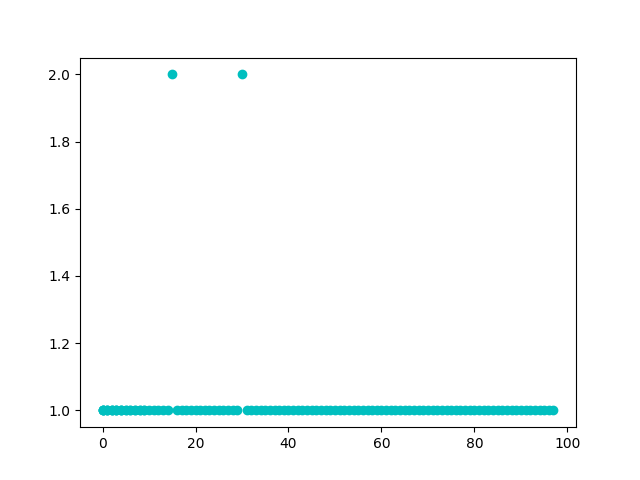
\includegraphics[width=0.45\textwidth]{img/grafico_indipendent_set_100_100.png} &
        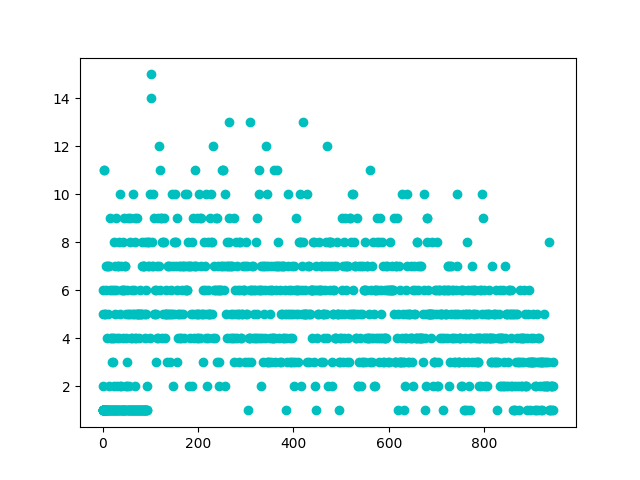
\includegraphics[width=0.45\textwidth]{img/grafico_indipendent_set_5000_100.png}
    \end{tabular}
    \caption{Numero di volte che viene generato un insieme in funzione del numero di esperimenti eseguiti}
\end{figure}

\newpage
\subsubsection{Generazione di colorazioni di grafi}

Il problema è definito da un grafo non orientato $ G = (V, E) $ con $ k $ nodi e da un insieme di colori $ Q = \{1, 2, \ldots, q\} $. Una $ q $-colorazione di $ G $ è una funzione $ f : V \rightarrow Q $ tale che, per ogni arco $ \{u, v\} \in E $, si ha $ f(u) \neq f(v) $. Denotiamo con $ Z_{G,q} $ il numero totale di $ q $-colorazioni di $ G $.

Quindi per il problema può essere costruito il campionatore di Gibbs associato impostando $R = Q$ 

\begin{equation}
    \pi(f)=\left\{\begin{array}{ll}
\frac{1}{Z_{G, q}} & \text { se } f \text { è una } q \text {-colorazione di } G \\
0 & \text { altrimenti }
\end{array}\right.
\end{equation}

$$S = \{ f \in Q^V \mid f \text{ è una } q\text{-colorazione di } G \}$$


Quindi, una volta fissata la $ q $-colorazione iniziale, la catena di Markov passa da uno stato all'altro mediante il seguente procedimento che modifica lo stato corrente $ f \in S $:

\begin{lstlisting}
Procedure NuovoStatoColorazione(f)
begin
    $\text{Scegli a caso } v \in V \text{ secondo la distribuzione uniforme}$
        $\text{Calcola } U_f(v) = \{ c \in Q : f(w) \neq c \text{ per ogni } w \text{ vicino di } v \} $
            ($\text{Nota che } U_f(v) \neq \emptyset \text{ poiché}  f(v) \in U_f(v) $)
    $\text{Scegli a caso c} \in U_f(v) \text{ secondo la distribuzione}$
    $ f(v) = c $
    $\textbf{return } f$
end
\end{lstlisting}

Denotando con $ P(f, g) $ la probabilità di andare in un passo dallo stato $ f $ allo stato $ g $ (per ogni coppia di $ q $-colorazioni $ f, g $ di $ G $), abbiamo che

\begin{equation*}
    P(f, g)=\left\{\begin{array}{ll}
0 & \begin{array}{c} \text { se } f \text { e } g \text { si differenziano per il valore }\\ \text{attribuito ad almeno } 2 \text { nodi } \end{array}\\
\frac{1}{k} \cdot \frac{1}{\sharp U_{f}(v)} & \begin{array}{c} \text { se } f \text { e } g \text { si differenziano per il valore }\\ \text{attribuito ad un solo nodo } v  \end{array} \\
    \sum_{v \in V} \frac{1}{k} \frac{1}{q-\sharp f(\operatorname{Adiacenza}(v))}>0 &  \begin{array}{c} \text{ se } f = g \end{array}
\end{array}\right. 
\end{equation*}

\begin{proposition}
\label{def:algebra}
La distribuzione $\pi$ è reversibile per la catena di Markov $ \{X_n\}$ definita sopra
\end{proposition}
\textit{Dimostrazione.}
Essendo la catena di Markov appena definita un esempio concreto di \textit{Campionatore di Gibbs} allora la proposizione è vera in quanto è vera anche la \hyperref[prp:gibbs_reversible]{Proposizione \ref*{prp:gibbs_reversible}}. 
Ricordiamo anche che per la \hyperref[prp:rev_staz]{Proposizione \ref*{prp:rev_staz}} allora la distribuzione è stazionaria per la catena $ \{X_n\} $

\begin{proposition}
La distribuzione $\pi$ è aperiodica per la catena di Markov $ \{X_n\}$ definita sopra

\end{proposition}

\begin{proof}

Basti notare che $ P(f, f) > 0 $ per ogni $q$-colorazione $f$ di $G$; infatti
$P(f, f)=\sum_{v \in V} \frac{1}{k} \frac{1}{q-\sharp f(\operatorname{Adiacenza}(v))}>0$, quindi è aperiodica per la \hyperref[prp:aperiodica]{Proposizione \ref*{prp:aperiodica}}

\end{proof}


\begin{proposition}
La catena  $ \{X_n\} $ che ha come matrice di transizione $ P = [P(A, B)]_{A,B \in S} $ è irriducibile (quindi ergodica) nel caso in cui $q \geq d + 2$ dove $d$ è il grado di $G$
\end{proposition}
\begin{proof}
Richiamando la \hyperref[def:irriducibile]{Definizione \ref*{def:irriducibile}}. la catena è irriducibile se per ogni stato (colorazione) $f, g \in S$ si ha che $F(f,g) > 0$
La dimostrazione è per induzione sul numero di nodi in cui $f$ e $g$ si differenziano

 \begin{itemize}
        \item{se $f =g$} \\ 
            siccome $P(f,f) > 0$ allora anche $F(f,f) > 0$
        \item{$\text { se } f \text { e } g  \text { si differenziano per il valore attribuito ad un solo nodo } v $}: \\ 
            In questo caso $P(f,g) = \frac{1}{k} \cdot \frac{1}{\sharp U_{f}(v)} > 0$, quindi $F(f,g) > 0$
        \item{$\text { se } f \text { e } g \text { si differenziano per il valore attribuito ad } n \text { nodi, con } n\geq 2$}: \\
        Sia $\{v_1, \dots, v_n\} \subseteq V$ per cui $\forall j \in \{1 \dots n\}, f(v_j) \neq g(v_j)$

        L'idea è quella di colore il colore  al nodo $v_n$ in $g(v_n)$, per fare questo però è necessario modificare il colore dei nodi adiacenti a $v_n$ che hanno come colore $g(v_n)$, l'insieme di questi nodi è  $\{v_{d_1}, \dots, v_{d_l}\} \subseteq \{v_1, \dots, v_n\}$, tenendo conto che $0 \leq l \leq d$.
        Quindi per ogni $i \in \{0 \dots l + 1\}$ definisco la colorazione $f_i$, nel seguente modo
        \begin{itemize}
            \item $i = 0$ \\ 
            $f_0 = f$ \vspace{14pt}

            \item $1 \leq i \leq l$ \\
            $\forall v \in V$ \\
            $f_i(v) = \left\{\begin{array}{ll}
                c \in U_{f_{i-1}} \setminus \{g(v_n) \} & \begin{array}{c} \text { se } v = v_{d_i}  \end{array}\\
                f_{i-1}(v) & \begin{array}{c} \text { altrimenti } \end{array}\\
        \end{array}\right. $ \\
            
            Nota che l'insieme $U_{f_{i-1}} \setminus \{g(v_n) \} $ non può essere vuoto, siccome per ipotesi $q \geq d + 2$ \vspace{14pt}


            \item $i = l+1$ \\
            $\forall v \in V$ \\
              $f_{l+1}(v) = \left\{\begin{array}{ll}
                g(v) & \begin{array}{c} \text { se } v = v_n \end{array}\\
                f_{l}(v) & \begin{array}{c} \text { altrimenti } \end{array}\\
        \end{array}\right. $ \\
        Notiamo che nel caso $v =v_n$ è sempre ammissibile il colore $g(v)$ perché è stato cambiato in $f_{l}$ per tutti i nodi $l$ adiacenti 
        \end{itemize}\vspace{14pt}

        Notiamo che $\forall i \in \{1 \dots l+1\}$ $f_{i-1}$ e $f_{i}$ differiscono al più di un nodo, quindi $P(f_{i-1},f_{i}) > 0 $ e questo significa che $F(f, f_n) > 0$ e siccome $f_{l+1}$ e $g$ si differenziano per il valore attribuito al più a $n-1$ nodi, si ha che $F(f_l,g) > 0$ per ipotesi induttiva. Quindi $F(f,g) \geq F(f, f_{l+1}) \cdot F(f_{l+1}, g) > 0$.

        Essendo la catena irriducibile, aperiodica ed essendo $\pi$ distribuzione stazionaria, per il \hyperref[thm:ergodic]{Teorema \ref*{thm:ergodic}} è ergodica
      

\end{itemize}
\end{proof}

\vspace{14pt}

\textbf{Implementazione Algoritmo e Risultati Finali} \\ \\
L'algoritmo Markov Chain Monte Carlo per generare una colorazione casuale di un grafo prevede che, partendo da uno stato qualsiasi della catena di Markov definita in precedenza, si compiano $n$ transazioni con $n$ abbastanza grande da garantire la completa casualità della colorazione generata. Quindi la procedura per generare la colorazione è la seguente

\begin{lstlisting}
Procedure GeneraColorazione(n)
begin
    $\text{calcola una }q\text{-colorazione }f \in S\text{ qualsiasi}$
    for $i = 1, \dots , n$ do
        begin
            $f$ := NuovoStatoColorazione($f$)
        end
    $\textbf{return} f$
end

\end{lstlisting}

L'algoritmo appena definito è stato implementato in Python, poi è stato eseguito sul seguente grafo: 

\begin{tikzpicture}[every node/.style={circle,draw}, node distance=1.5cm]

\node[rectangle, draw=none, fill=none, font=\bfseries\Large] (title) at (5,2.5) {}; %non serve a niente ma senza il disegno diventa spostato

% Posizioni dei nodi
\node (a) at (0,0) {a};
\node (b) at (2,1) {b};
\node (c) at (2,-1) {c};
\node (d) at (2,0) {d};
\node (e) at (4,0) {e};
\node (f) at (6,0) {f};

% Archi
\draw (a) -- (b);
\draw (a) -- (c);
\draw (a) -- (d);
\draw (b) -- (d);
\draw (b) -- (e);
\draw (c) -- (d);
\draw (c) -- (e);
\draw (d) -- (e);
\draw (e) -- (f);

\end{tikzpicture}
\\
Ed ecco un paio di esempi di colorazioni generate: 

\begin{tikzpicture}[every node/.style={circle,draw}, node distance=1.5cm]

\node[rectangle, draw=none, fill=none, font=\bfseries\Large] (title) at (5,2.5) {}; %non serve a niente ma senza il disegno diventa spostato

\node (a) at (0,0) {5};
\node (b) at (2,1) {6};
\node (c) at (2,-1) {4};
\node (d) at (2,0) {3};
\node (e) at (4,0) {1};
\node (f) at (6,0) {5};

% Archi
\draw (a) -- (b);
\draw (a) -- (c);
\draw (a) -- (d);
\draw (b) -- (d);
\draw (b) -- (e);
\draw (c) -- (d);
\draw (c) -- (e);
\draw (d) -- (e);
\draw (e) -- (f);

\end{tikzpicture}
\\


\begin{tikzpicture}[every node/.style={circle,draw}, node distance=1.5cm]

\node[rectangle, draw=none, fill=none, font=\bfseries\Large] (title) at (5,2.5) {}; %non serve a niente ma senza il disegno diventa spostato

\node (a) at (0,0) {4};
\node (b) at (2,1) {2};
\node (c) at (2,-1) {6};
\node (d) at (2,0) {3};
\node (e) at (4,0) {1};
\node (f) at (6,0) {3};

% Archi
\draw (a) -- (b);
\draw (a) -- (c);
\draw (a) -- (d);
\draw (b) -- (d);
\draw (b) -- (e);
\draw (c) -- (d);
\draw (c) -- (e);
\draw (d) -- (e);
\draw (e) -- (f);


\end{tikzpicture}
\\


Il codice dell'algoritmo appena definito è stato implementato in Python e viene eseguito sul grafo mostrato a inizio capitolo, e qui vengono mostrati i risultati delle esecuzioni, su test al variare del numero dei passi $n$ e generando $100000$ colorazioni per ogni test (un numero arbitrario che però è molto maggiore al numero di colorazioni totali). Si può notare che all'aumentare di $n$ la frequenza di colorazioni generate si allineano alla che avrebbero se fossero generate con distribuzione uniforme, dando prova empirica dell'ergodicità della catena di Markov.

\begin{figure}[!ht]
    \centering
    \begin{minipage}{0.45\textwidth}
        \centering
        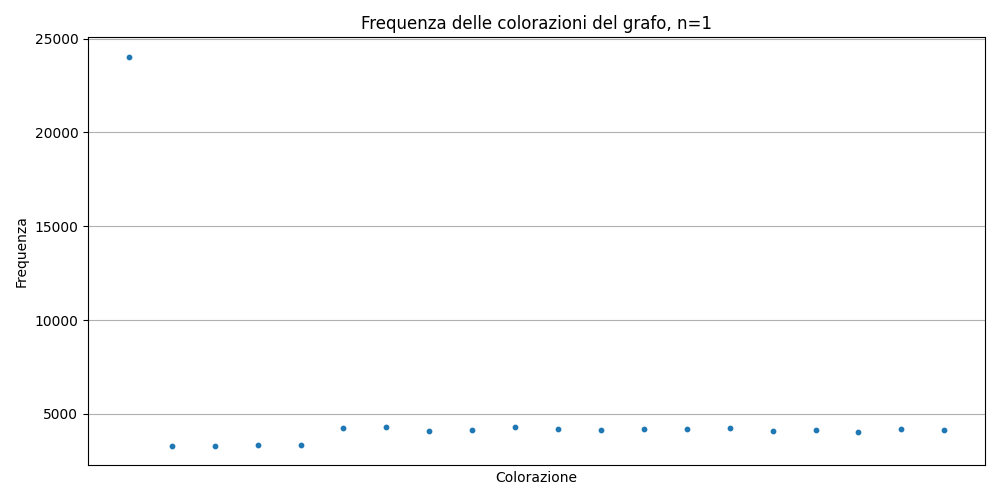
\includegraphics[width=\linewidth]{img/grafico_frequenza_colorazioni_n1.png}
        \caption{Frequenza delle colorazioni del grafo per n = 1}
        \label{fig:immagine1}
    \end{minipage}\hfill
    \begin{minipage}{0.45\textwidth}
        \centering
        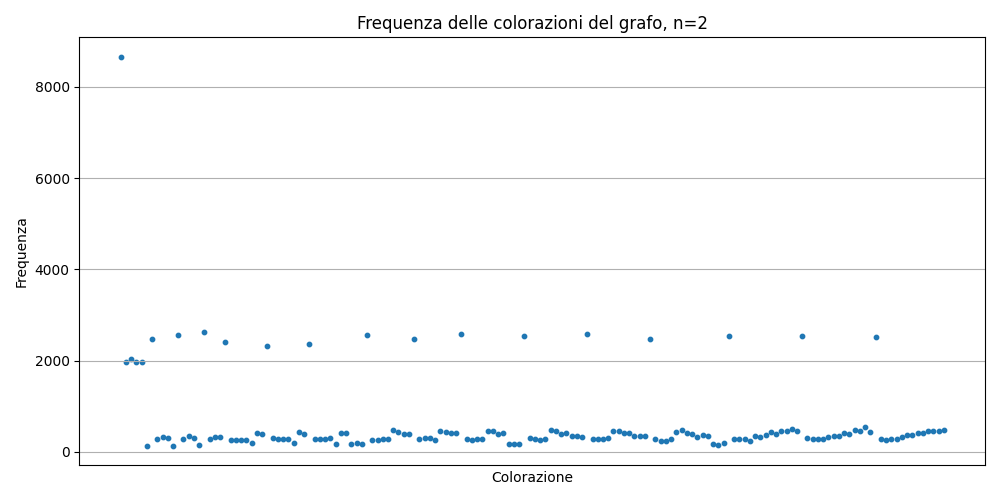
\includegraphics[width=\linewidth]{img/grafico_frequenza_colorazioni_n2.png}
        \caption{Frequenza delle colorazioni del grafo per n = 2}
        \label{fig:immagine2}
    \end{minipage}
\end{figure}

\begin{figure}[!ht]
    \centering
    \begin{minipage}{0.45\textwidth}
        \centering
        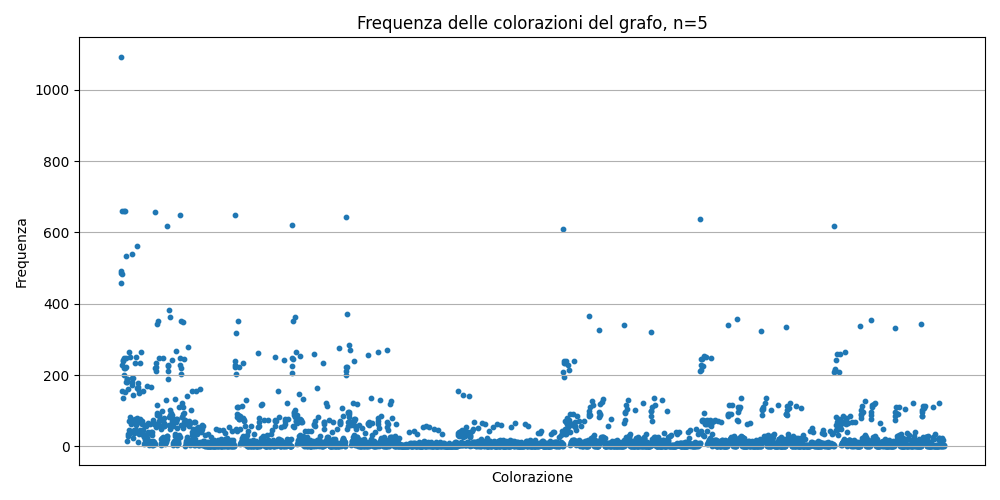
\includegraphics[width=\linewidth]{img/grafico_frequenza_colorazioni_n5.png}
        \caption{Frequenza delle colorazioni del grafo per n = 5}
        \label{fig:immagine1}
    \end{minipage}\hfill
    \begin{minipage}{0.45\textwidth}
        \centering
        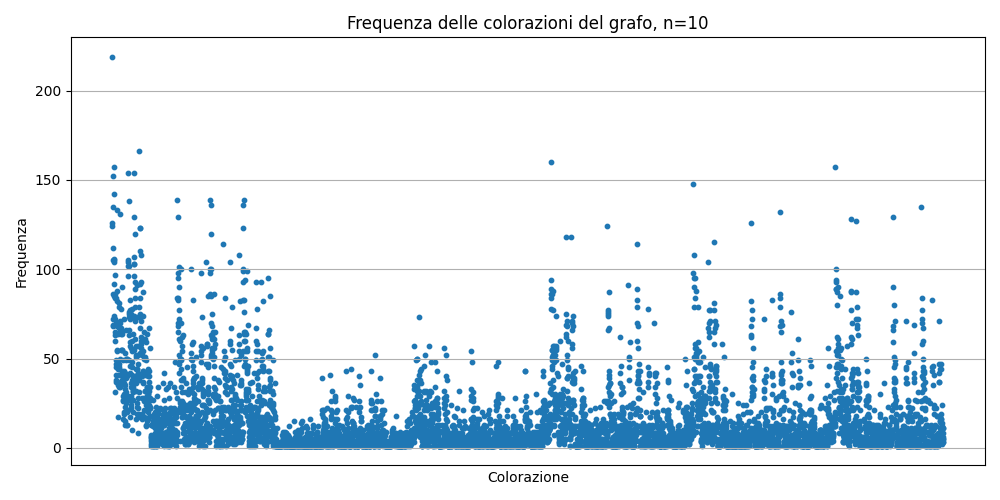
\includegraphics[width=\linewidth]{img/grafico_frequenza_colorazioni_n10.png}
        \caption{Frequenza delle colorazioni del grafo per n = 10}
        \label{fig:immagine2}
    \end{minipage}
\end{figure}

\begin{figure}[!ht]
    \centering
    \begin{minipage}{0.45\textwidth}
        \centering
        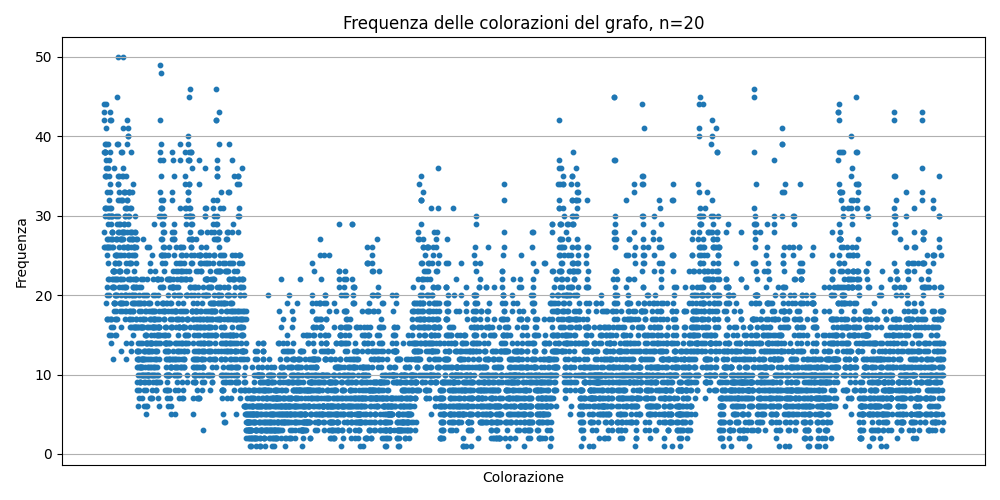
\includegraphics[width=\linewidth]{img/grafico_frequenza_colorazioni_n20.png}
        \caption{Frequenza delle colorazioni del grafo per n = 20}
        \label{fig:immagine1}
    \end{minipage}\hfill
    \begin{minipage}{0.45\textwidth}
        \centering
        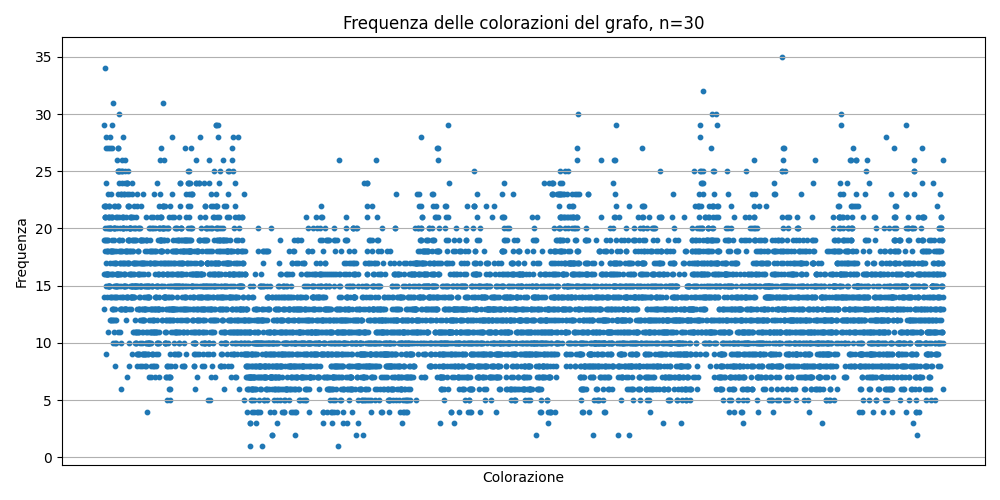
\includegraphics[width=\linewidth]{img/grafico_frequenza_colorazioni_n30.png}
        \caption{Frequenza delle colorazioni del grafo per n = 30}
        \label{fig:immagine2}
    \end{minipage}
\end{figure}

\begin{figure}[!ht]
    \centering
    \begin{minipage}{0.45\textwidth}
        \centering
        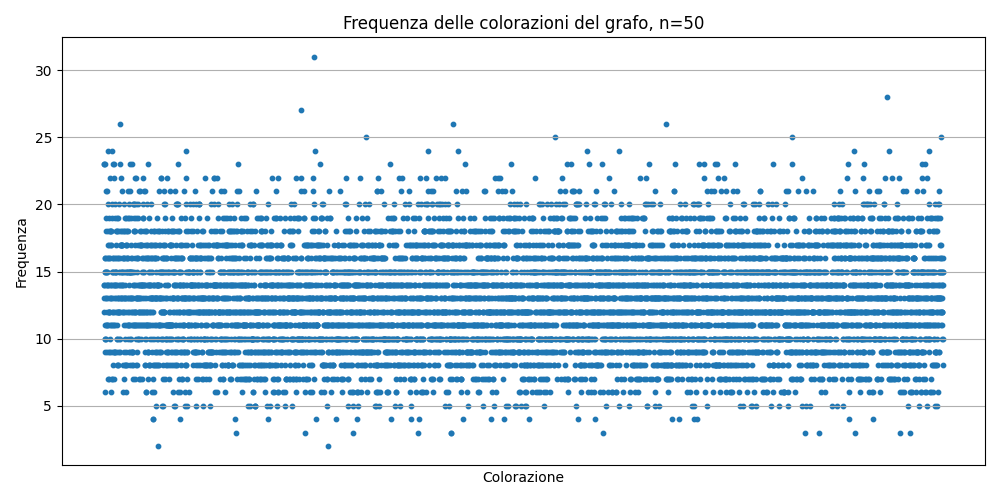
\includegraphics[width=\linewidth]{img/grafico_frequenza_colorazioni_n50.png}
        \caption{Frequenza delle colorazioni del grafo per n = 50}
        \label{fig:immagine1}
    \end{minipage}\hfill
    \begin{minipage}{0.45\textwidth}
        \centering
        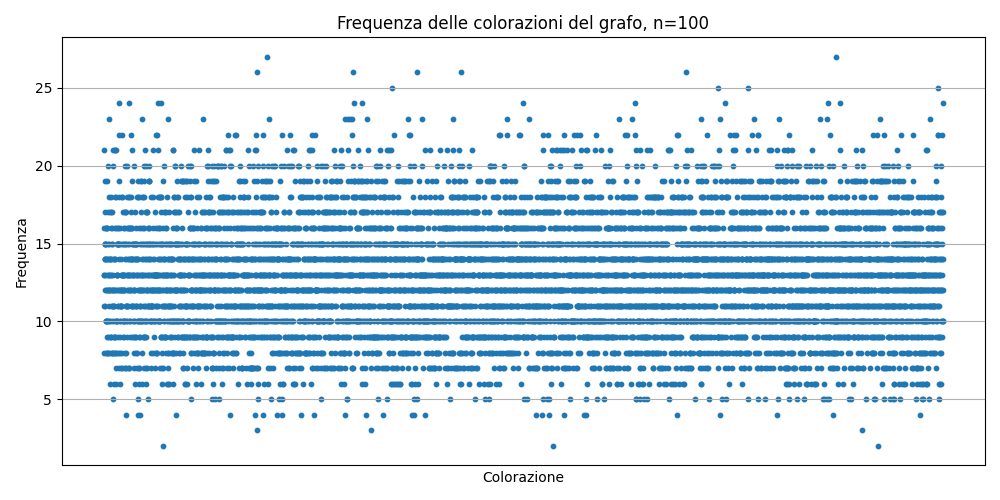
\includegraphics[width=\linewidth]{img/grafico_frequenza_colorazioni_n100.png}
        \caption{Frequenza delle colorazioni del grafo per n = 100}
        \label{fig:immagine2}
    \end{minipage}
\end{figure}

\newpage
\section{Possibili sviluppi futuri}

Possibili approfondimenti sul tema potrebbero riguardare l'analisi e implementazione di altri tipi di algoritmi Markov Chain Monte Carlo, diversi da Campionatori di Gibbs, come l'algoritmo di Metropolis; oppure sarebbero interessanti approfondimenti relativi alla velocità di convergenza degli algoritmi appena mostrati. Qui sotto riportiamo una breve descrizione di questi due argomenti. 


\subsection{Algoritmo di Metropolis}

Le catene di Markov trovano un'ampia gamma di applicazioni, e un metodo classico per la generazione casuale basato su di esse \`e l'algoritmo di Metropolis. 
Questo algoritmo rappresenta un procedimento generale per la generazione casuale di un elemento all'interno di un 
insieme finito $V$ secondo una distribuzione di probabilit\`a $\pi$ fissata (con $\pi(S_i) > 0$ per ogni $S_i \in V$).

Il metodo prevede la definizione di un grafo non orientato $G = (V,E)$, dove $V$ è l'insieme degli stati, che deve essere connesso e avere un grado massimo limitato. 
Se denotiamo con \( d_i \) il grado del generico nodo \( S_i \in V \), possiamo definire la probabilità \( P(i,j) \) di passare da un nodo \( S_i \) a un nodo \( S_j \) nel modo seguente:

\[
P(i,j) =
\begin{cases}
0 & \text{se } i \neq j \text{ e } \{i,j\} \notin E \\
\frac{1}{d_i} \cdot \min\left\{ \frac{\pi_j d_i}{\pi_i d_j}, 1 \right\} & \text{se } \{i,j\} \in E \\
1 - \frac{1}{d_i} \cdot \sum_{\ell : \{i,\ell\} \in E} \min\left\{ \frac{\pi_\ell d_i}{\pi_i d_\ell}, 1 \right\} & \text{se } i = j
\end{cases}
\].

Qualora la catena soddisfi le condizioni di ergodicit\`a e periodicit\`a, possiamo quindi adottare il solito criterio: simuliamo la catena a partire da uno stato qualsiasi per un numero sufficientemente grande di passi e restituiamo il valore dello stato raggiunto. Al crescere del numero di passi sappiamo che la probabilit\`a di restituire un valore $i$ approssima $\pi_i$, per ogni $S_i \in V $

\subsection{Analisi velocità di convergenza}
Per valutare l'efficienza degli algoritmi Markov Chain Monte Carlo (MCMC), come quelli per la generazione casuale di insiemi indipendenti o di colorazioni di grafi, è fondamentale analizzare la loro velocità di convergenza alla distribuzione di probabilità desiderata. Questa analisi mira a determinare quanti passi della catena di Markov sono necessari affinché la distribuzione di probabilità dello stato corrente si approssimi sufficientemente alla distribuzione stazionaria $\pi$. 

La misura chiave per questa velocità è il mixing time $\tau(\epsilon)$, che indica il numero minimo di passi dopo il quale la distanza di variazione totale tra la distribuzione della catena e $\pi$ è minore o uguale a un errore prefissato $\epsilon$.

Un metodo potente per stimare il mixing time è il metodo dell'accoppiamento (coupling method). Questo approccio implica la costruzione di due catene di Markov identiche che partono da stati diversi ma evolvono in parallelo, e si concentra sulla probabilità che le due catene si incontrino. Se le catene si incontrano rapidamente, si può dedurre che il loro mixing time è piccolo.
Purtroppo il metodo dell’accoppiamento meriterebbe un approfondimento a parte, che esula dallo scopo di questo testo.

\begin{thebibliography}{9}

\bibitem{testo1}
Massimiliano Goldwurm,
\textit{Catene di Markov e applicazioni algoritmiche}.
2024.

\bibitem{testo2}
Rick Durrett,
\textit{Essentials of Stochastic Processes}.
2011.

\bibitem{testo3qweeeeeeeeeeeee}
M. Jerrum,
\textit{A very simple algorithm for estimating the number of k-colorings of a low-
degree graph}.
1994.


\end{thebibliography}


\end{document}
